\documentclass[12pt, a4paper]{article} % 设置字体大小和纸张类型
\usepackage{fontspec}
\setmainfont{Times New Roman}

\usepackage{booktabs} % 支持更专业的表格线条
\usepackage{ctex}
\usepackage{caption} % 插图和表格的标题格式
\usepackage{amsmath, amsfonts, amssymb} % 数学公式支持
\usepackage{graphicx} % 插入图片
\usepackage{hyperref} % 超链接支持
\usepackage{hypcap} % 修正超链接指向的图片位置
\usepackage[a4paper, margin=2.5cm]{geometry}
\usepackage{titlesec}
\usepackage{fmtcount} % 用于数字到中文的转换
\usepackage{enumitem} % 加载 enumitem 宏包
\usepackage{multirow} % 支持多行单元格
\usepackage{diagbox}
\usepackage{makecell} % 支持单元格内换行
\usepackage{tikz}
\usepackage{makecell}
\usepackage{unicode-math}
\usepackage{bookmark} % 书签支持
\setmathfont{Latin Modern Math}



\renewcommand{\thesection}{\chinese{section}、}
\renewcommand{\thesubsection}{\arabic{subsection}.}


\begin{document}

\sloppy

\begin{titlepage}
    \newgeometry{left=0cm, right=0cm, top=0cm, bottom=0cm}
    \centering
    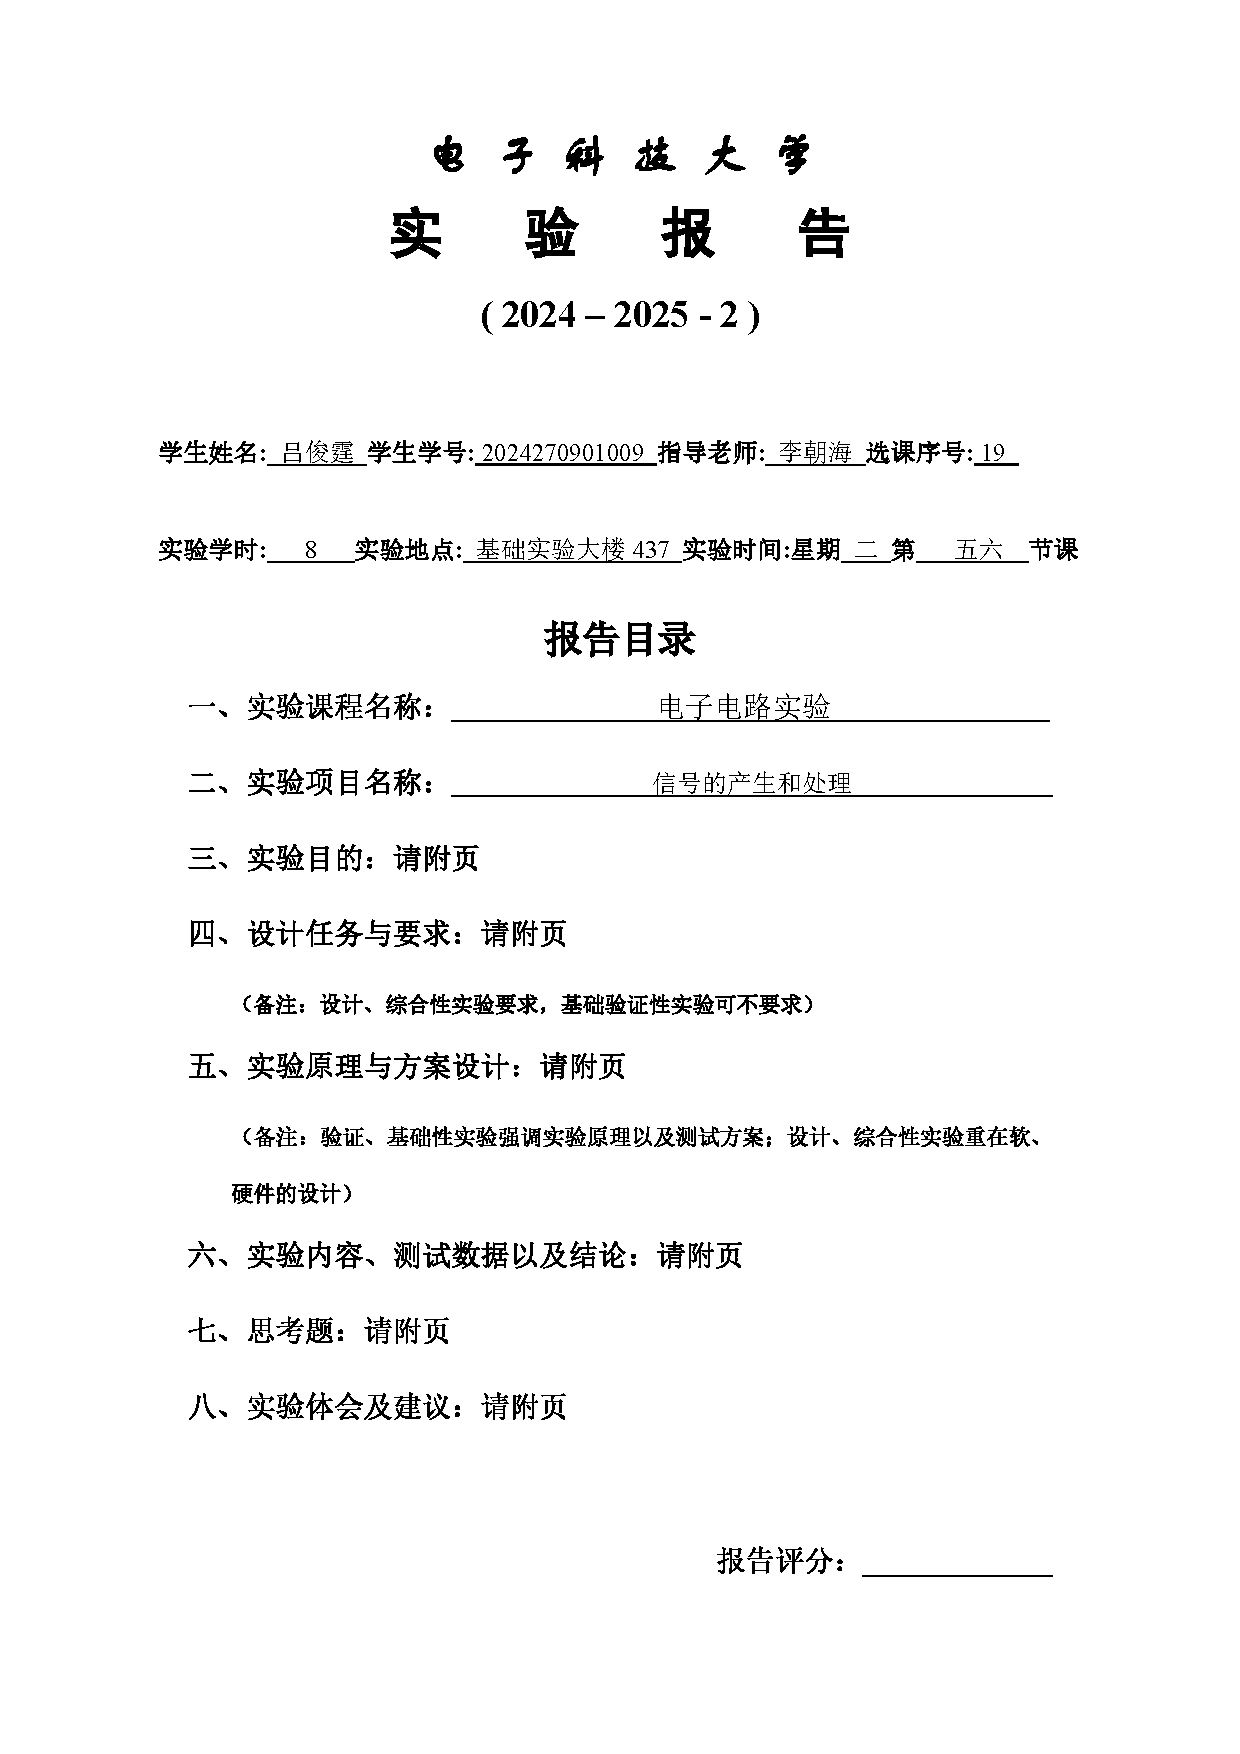
\includegraphics[page=1, width=0.9\textwidth, keepaspectratio]{image/实验报告撰写封面.pdf}
    \restoregeometry
\end{titlepage}

\setcounter{section}{2}

\section{实验目的}

\begin{enumerate}[leftmargin=50pt,label=(\arabic*)] % 设置序号格式为(1)
    \item 理解函数信号的产生原理
    \item 掌握利用继承运放单元电路进行电子电路系统设计的方法
    \item 掌握电路调试和指标测试技术
\end{enumerate}

\section{设计任务与要求}

用给定的运算放大器设计并制作一个信号产生与处理电路

设计要求如图所示,设计制作一个方波产生器输出方波,再与三角波相叠加输出一个复合信号,再经过低通滤波器输出一个正弦波信号。

\begin{figure}[th]
    \centering
    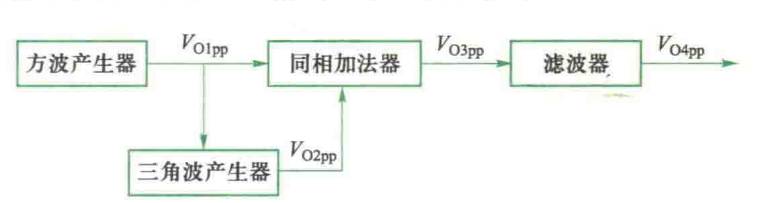
\includegraphics[width=0.8\textwidth]{image/1.png}
    \caption{实验电路图}
    \label{fig:实验电路图}
\end{figure}

设计要求如下:

(1) 方波产生器输出方波信号参数要求:$ V_{o1_{pp}} = 4V$, 误差为$ \pm 5\% $, f = 5kHz$\pm 100Hz$, 波形无明显失真;

(2) 三角波产生器输出三角波信号参数要求:$ V_{o2_{pp}} = 4V$, 误差为$ \pm 5\% $, f = 5kHz$\pm 100Hz$, 波形无明显失真;

(3) 同相加法器输出复合信号参数要求:$ V_{o3_{pp}} = 8V$, 误差为$ \pm 5\% $, f = 5kHz$\pm 100Hz$, 波形无明显失真;

(4) 滤波器输出正弦波信号参数要求:$ V_{o4_{pp}} = 4V$, 误差为$ \pm 5\% $, f = 5kHz$\pm 100Hz$, 波形无明显失真。

(5) 要求预留方波$V_{o1_{pp}}$、三角波$V_{o2_{pp}}$、复合信号$V_{o3_{pp}}$和正弦波$V_{o4_{pp}}$的输出端口,便于后续测试。

(6) 设计报告需给出方案设计,详细电路图,仿真结果和实物测试数据波形
\section{实验原理与方案设计}
\subsection{实验原理}
\section{实验内容、测试数据以及结论}

\subsection{实验内容}

\subsection{实验结论}
……
\section{思考题}
\subsection{题面}
\begin{enumerate}[leftmargin=50pt,label=(\arabic*)] % 设置序号格式为(1)
    \item text

\end{enumerate}
\subsection{回答}

\begin{enumerate}[leftmargin=50pt,label=(\arabic*)] % 设置序号格式为(1)
    \item text
\end{enumerate}

\section{实验体会及建议}
\subsection{实验体会}
测量时应注意小心调试仪器, 尽量将读数稳定在误差允许范围内进行读数。
\subsection{建议}
注意电源正负极的接入, 防止反接造成仪器损坏, 注意正负电压的接入, 防止反接造成仪器损坏。

\end{document}
